\subsection{Interface}
	These are the server side scripts that will be used across the website.

	\emph{Constants}
	\begin{itemize}
		\item Header
		\begin{itemize}
			\item session\_start();
			\item Doctype
			\item meta tags
			\begin{itemize}
				\item description
				\item Keywords
				\item authir
				\item content type
				\item CSS links
				\item Font link
				\item validation.js
				\item \$title
			\end{itemize}
			\item Header/Div
			\begin{itemize}
				\item Logo
			\end{itemize}
		\end{itemize}

		\item Nav
		\begin{itemize}
			\item Nav
			\item include`breadcrumbs';
		\end{itemize}
		\item Footer 
		\begin{itemize}
			\item Site map link 
			\item Icon
		\end{itemize}
			
		\item config.php
		\begin{itemize}
			%%\$host = \"\";
			%%\$port \= \"\";
			%%\$user \= \"\";
			%%\$password \= \"\";
			%%\$dbname \= "";
			%%mysql \= new mysql(\$...)
			%%die statements
			\item Address of Server
			\item Admin Password
		\end{itemize}

		\item Index
		\begin{itemize}
			\item \$title
			\item include `header.php';
			\item include `nav.php';
			\item text
			\item include `simple\_search.php';
			\item text
			\begin{itemize}
				\item app link
			\end{itemize}
			\item include `footer.php';
		\end{itemize}	

		\item plants
		\begin{itemize}
			\item include `config.php';
			\item \$title
			\item include `header.php';
			\item include `nav.php';
			\item add\_plant\_record link
			\item include `advanced\_search.php';
			\item include `plant\_db\_declare.php';
			\item include `plant\_sorting.php';
			\item include `footer.php';
		\end{itemize}
		\item add\_plants\_record
		\begin{itemize}
			\item include `config.php';
			\item \$title
			\item include `header.php';
			\item include `nav.php';
			\item form(input)
			\item if no image uploaded, default image else uploaded image
			\item include `upload\_image.php';
			\item include `save\_record.php';
			\item a href `plants.php' cancel
			\item include `footer.php';
		\end{itemize}
		
		\item plants\_record
		\begin{itemize}
			\item include `config.php';
			\item \$title
			\item include `header.php';
			\item include `nav.php';
			\item \$specific record details
			\item a href `edit\_plant\_record.php' edit
			\item a href `delete\_plant\_record.php' remove
			\begin{itemize}
				\item delete prompt js
			\end{itemize}
			\item individual record photo or default image
			\item a href `plants.php' where to find
			\begin{itemize}
				\item (plant\_map.js)
			\end{itemize}
			\item include `footer.php';
		\end{itemize}

		\item edit\_record
		\begin{itemize}
			\item include `config.php';
			\item \$title
			\item include `header.php';
			\item include `nav.php';
			\item include `breadcrumbs.php';
			\item \$individual record
			\item a href `edit\_plant\_record.php' edit
			\item a href `delete\_plant\_record.php' remove
			\item \$individual record photo
			\item a href `plants.php' where to find
			\begin{itemize}
				\item (plant\_map.js)
			\end{itemize}
			\item include `footer.php';
		\end{itemize}
	\end{itemize}

\subsection{Detailed design}

	\subsubsection{timeout.php}
		Time out is essentially a script that will unset a specific session when no activity has taken place, display and alert message, which once confirmed will send the user back to the plant list page. This will mainly be included when adding or editing records, as if the computer is left alone, then anyone could distort the record information.

	\subsubsection{plants.php}
		The plants page is where the list of plants are going to be displayed. The page will require the connection to the database through the config file, and it must include the html pages header.php, nav.php and the footer.php files.  The page will also have its own heading that will be created by a variable, will be declared above the header.php include, where the header will have \$title so it can be adjusted easily. The main content area below the navigation, which is then split into two. The first section is where the user will be able to sort the database records to their specific criteria. This sorting script will be placed in a separate file. The other half, is the main part of the page. In this section, the user can select a link that will allow them to create a new plant record and store it in the database. Under that, there is an advanced search, which will display records that comes under the criteria of their search input. This will also be in a separate script. This search will allow the user to not have to scroll through the long list of records. The plants are split into their scientific name and their common name. Once they are clicked, then they are taken to the plants individual record. The database itself is going to be called and declared from a separate script, where it will then place them into a table, which will present the plant lists.

	\subsubsection{db\_declare.php}
		This script is basically where and how the plant list will be created and how it will be represented. Firstly, the table will have to be created, which will have a div attached to it. Then the scientific and common headings will be created. Once this has been created, an SQL statement will be used, making a handle onto the database connection, where it will select all the fields by using.  We can then use the handle from the SQL statement to write out the database, using \texttt{while(\$row = pg\_fetch\_array (\$res))} and then defining the cells by calling them by \texttt{\$row[`dbcolumn']} inside of td tags.  Each of these rows will be links to the page that has their information on. The table is then closed. The script does require config.php, but this is already included in plants.php

	\subsubsection{Plant location}
		When showing the specific location of the plant, we will be using the google maps JavaScript API. To use this we will have to gain an API key from google;once we have access, we must activate the Google Maps API v3. To get the API key, we must give it some information about the website, such as the web address. Because we will be testing it on another server, we will register it to that site first, which we can change to the server we will be using it on later on at the final part of the project.

		Implementing the code must start with giving the script source, included into the HTML head, where the API key must be inserted.  Then a new JavaScript script will be created, stating an initialize function. This will be made up of a variable mapProp, where it will specify all of the options for the map, such as where to center the map, how close are we going to zoom in on the location and what type of map is it going to be, such as Roadmap and Terrain, which we will be using HYBRID, as it allows to see a combination of the roads and the scenery, which may be useful to a botanist trying to find the specific plant. In these options however, is the lat/lang input, which will locate where the plant is. Because this depends on the location of the plant that will be displayed, we will have to use a variable that will get the latitude and longitude from the record and place it in the variable so it can there be used to display its location. After these options have been defined, the mapProp variable is closed, and the map is then created through creating a new map variable, which will assign itself to a div depending on its ID. The script must then be closed. To display this, in the body, there must be a div with the same ID stated in the script. 

	\subsubsection{config.php}
		config will open a link to the mysql database at the start of each new session, all changes to records and searches are reliant on this script.
		\begin{verbatim}
			$conn = mysql_connect(host=<localhost> 
			port=3306 dbname=<nameofdatabase> 
			user=<uid> password=<password>);
		\end{verbatim}
		The script will also include a few lines closing the link to the database at the end of the session as not to produce more connections to the database than needed.

	\subsubsection{plant\_sorting.php}
		The plant data can be sorted in multiple different ways there will be a default sort using SORT\_REGULAR however the options of SORT\_STRING and SORT\_NUMERIC will also be available as required. The script will provide the user with an option of how they wish to sort the data.

	\subsubsection{simple\_search.php}
		The simple search script will search the database for a string matching the users input, all entries in the database containing that string will be returned. It will require a connection to the database from config.php, if there is no connection then the script will return an error message to notify the user of a problem with the connection to the database.

	\subsubsection{advanced\_search.php}
		The script for advanced search will allow for searches by string, ID, data type, location and user. The user should select their search type before inputting, the results shall be returned unless no result is found or there is an issue with the connection to the database in which case an error message shall be returned to the user. 

	\subsubsection{edit\_plant\_record.php}
		This script will take data input from the client side to form an update in an object oriented way. The update will set the field to be updated to the new data. The script will query if the connection to the server is valid before committing the changes, it will also return a confirmation to the user that the record has been updated or that there was a problem connecting to the server (they have timed out) so they can try again.

	\subsubsection{delete\_plant\_record.php}
		The script for deleting a record will be very straight forward, using an object oriented approach the script will request for the record to be deleted by using its ID. Much like the edit this script will return a confirmation to the user that the record has successfully been deleted or that there was a problem with the connection to the server.

	\subsubsection{upload\_image.php}
		This script should prompt the user to choose an image file to upload first, when an image file has been selected an upload function will collect the data about the file where it can be validated to check it matches the requirements we have set (eg: file type and size). The image file, if compatible, will be uploaded and the script will return a success message, otherwise a message will be returned to the user explaining which parameter is incorrect or if there is an issue with the connection to the server.

	\subsubsection{regex validation}
		validation will be done on the client side using javascript and regular expressions. Doing this allows us to use an onchange method when the user is inputting data with fixed parameters, such as what characters can be used, without putting extra load on the server.

	\subsubsection{Index.php}
		The index script will be the home page for the web site, allowing users to read about the Botany Project, navigate the web site, search for a plant and download the app. There will be a header at the top of the page containing the Botany Group Project title and an image of the logo. The banner will be customised using CSS. Underneath there will be a navigation bar using the nav.php script. Below this there will be two text boxes which will be achieved using the echo function and will be customised to have a white background using CSS. Between the texts there will be a search bar controlled by simple\_search.php. At the bottom the footer.php will be included. A background image will be used for the homepage.

	\subsubsection{Header.php}
		The header will be responsible for creating a session for the user. The header script will be responsible used to declare the doctype and meta tags such as description, keywords, content type, CSS and font links, validation.js and title. 

	\subsubsection{footer.php}
		The footer will contain the site map link allowing users to access all the pages of the website. There will also be an image of the logo in the centre of footer.

	\subsubsection{nav.php}
		The navigation bar provides an easy reference for the contents of the web site and enables the user to navigate the web site conveniently. This will be achieved by attaching a div class to the navigation text with a href attribute, linking it to the corresponding pages. CSS will be used to style the navigation bar and links accordingly with the Web user interface design. Underneath there will be breadcrumbs included using the breadcrumbs script.

	\subsubsection{Edit/add record}
		Upon selecting an individual plant from the database, the plant along with its attributes and an image will be displayed by pulling it from the database using SQL. The user can find where to locate the plant by clicking the ‘Where to find’ button which will run the plant\_map.js script, loading Google maps javascript API. The user can then edit the plant’s information by clicking the edit button supplied, running the edit\_plant\_record.php script, loading the Edit Record page. This page will use the config.php script to form a database connection that will insert a table, ready to retrieve and print the selected fields of the plant chosen by the user. This will be achieved using pg\_query; selecting the required fields and echoing a table. A while loop will be used to read and  pull data from the database. Users can then edit plant information by filling in the form with the attributes assigned to a plant. The form is to be validated using javascript, identifying the required fields. If a required field is left blank, an alert will pop up requesting the user to fill the field in. The image can also be updated by clicking the supplied ‘Upload Image’ submit button, running the upload\_image.php script. Once the form has been edited by the user, they can then save the record using the Save button linked to the save\_record.php script. This will update the database with the new edited record. Users will also be given the option to add new plant records to the database. This page will be the same as the Edit Record page but with a blank form for the user to fill in.

	\subsubsection{delete record}
		Users are given the option to delete a specific plant record. A ‘remove’ button linked to the delete\_plant\_record.php script will be supplied to do this.

	\subsubsection{delete confirmation pop up}
		If a user clicks the remove button, a javascript alert pop up will be displayed confirming the deletion of a record. This has been included to avoid accidental deletions.

\begin{landscape}
    \begin{figure}
        \centering
        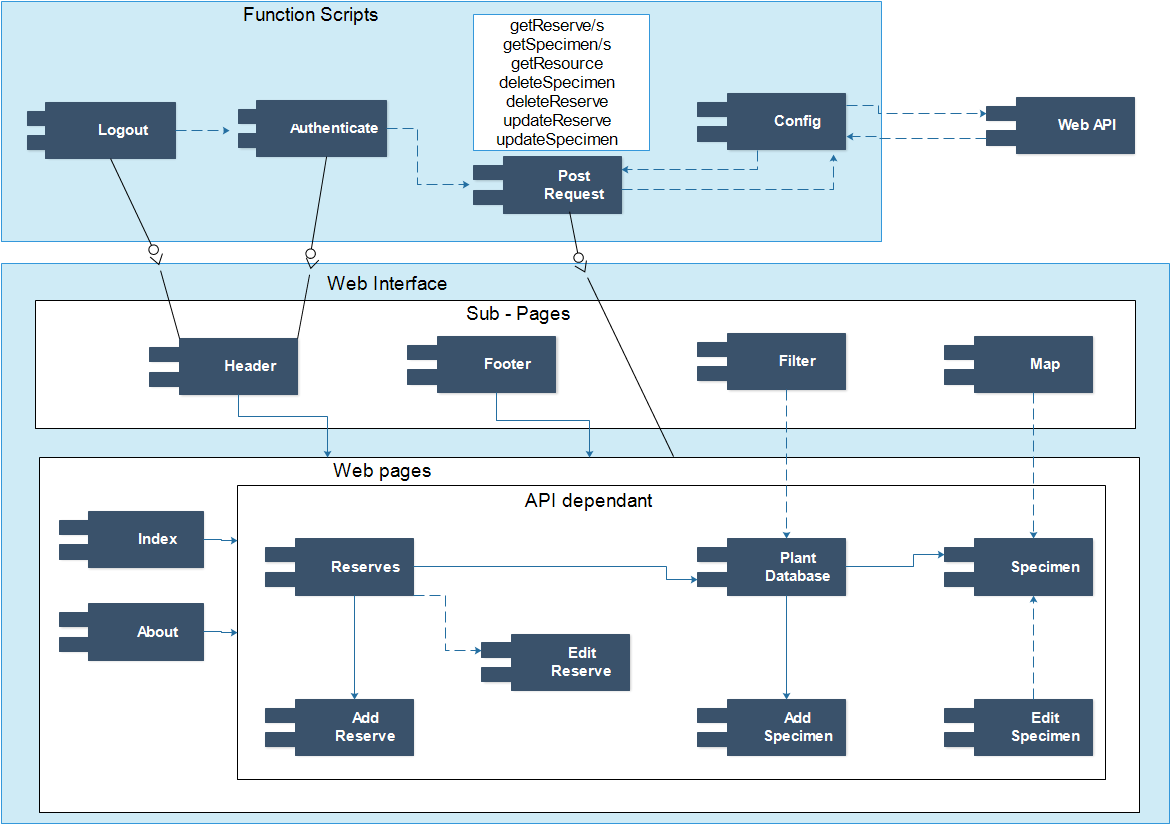
\includegraphics[scale=1]{web/webComponentDiagram.png}
        \caption{Web component Diagram}
        \label{fig:webComponentDiagram}
    \end{figure}
\end{landscape}


